\documentclass[aspectratio=1610]{beamer}
\usetheme{KTH}
\usepackage[utf8]{inputenc}
\usepackage[T1]{fontenc}
\usepackage[format=hang]{caption}
\usepackage{subcaption}
\captionsetup{font=normalsize,labelfont={bf,sf}}
\captionsetup[sub]{font={small}, textfont={normalfont}, labelfont={bf,sf}}
\usepackage{indentfirst}
\usepackage{pgfplots}
\pgfplotsset{compat=1.14}
\usepackage[export]{adjustbox}
\usepackage{tikz}
\usetikzlibrary{shapes,arrows.meta,positioning,automata}
\usepackage{libertine}
\usepackage{sourcecodepro}
\usepackage{todonotes}
\usepackage{wrapfig}

\usepackage[style=ieee,
backend=bibtex,
sorting=none,
sortcites,
maxbibnames=1,
minbibnames=1,
maxcitenames=2, 
mincitenames=1]{biblatex}
\AtBeginBibliography{\footnotesize}
\addbibresource{bibliography.bib}

\newcommand{\kthaffil}{\textsuperscript{\textdagger}}
\newcommand{\cmuaffil}{\textsuperscript{\textdaggerdbl}}

\begin{document}
\startpage
%%%%%%%%%%%%%%%%%%%%%%%%%%%%%%%%%%%%%%%%%%%%%%%%%%%%%%%%%%%%
\begin{frame}{}
    \begin{center}
        \begin{LARGE}
            \textbf{EdgeDroid}\\
        \end{LARGE}
        \emph{An Experimental Approach to Benchmarking Human-in-the-Loop Applications}\\
        \vspace{0.02\textheight}
        {\footnotesize \underline{M. Olguín Muñoz}\kthaffil, J. Wang\cmuaffil, M. Satyanarayanan\cmuaffil and J. Gross\kthaffil\\
            \vspace{0.02\textheight}
            \kthaffil~KTH Royal Institute of Technology\\
            \cmuaffil~Carnegie Mellon University\\}
    \end{center}

    \vspace{0.04\textheight}

    \begin{tiny}
        \raggedleft%
        \emph{HotMobile'19 Session 5: February 28\textsuperscript{th} 2019, Santa Cruz, CA}\\
    \end{tiny}
\end{frame}

\normalpage
\begin{frame}{Outline}
    \tableofcontents[hideallsubsections]
\end{frame}

\section{Introduction \& Background}
\subsection{Human-in-the-Loop Applications}
\begin{frame}
    \onslide<2->{\begin{columns}[onlytextwidth]
        \begin{column}{.335\linewidth}%filler
        \end{column}%
        \begin{column}{.1\linewidth}
            \centering%
            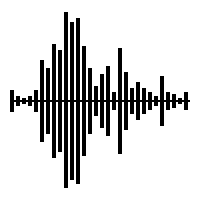
\includegraphics[width=\linewidth]{img/sound_wave.png}
        \end{column}%
        \begin{column}{.01\linewidth}
        \end{column}%
        \begin{column}{.1\linewidth}
            \centering%
            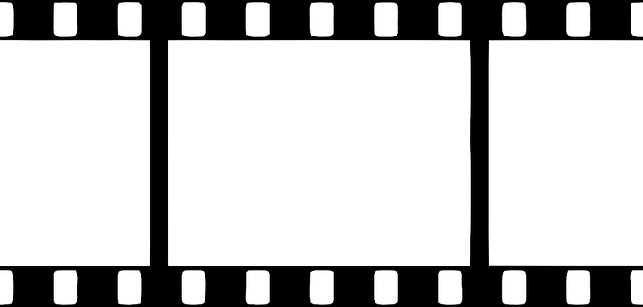
\includegraphics[width=\linewidth]{img/film.png}
        \end{column}%
        \begin{column}{.01\linewidth}
        \end{column}%
        \begin{column}{.1\linewidth}
            \centering%
            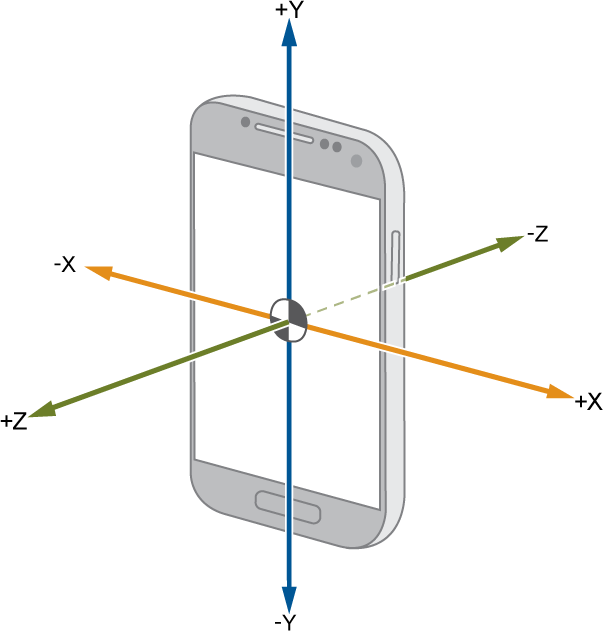
\includegraphics[width=\linewidth]{img/accel.png}
        \end{column}%
        \begin{column}{.335\linewidth}%filler
        \end{column}%
    \end{columns}}%
    \begin{columns}[onlytextwidth]
        \begin{column}{.25\linewidth}
            \centering%
            \onslide<3->{
                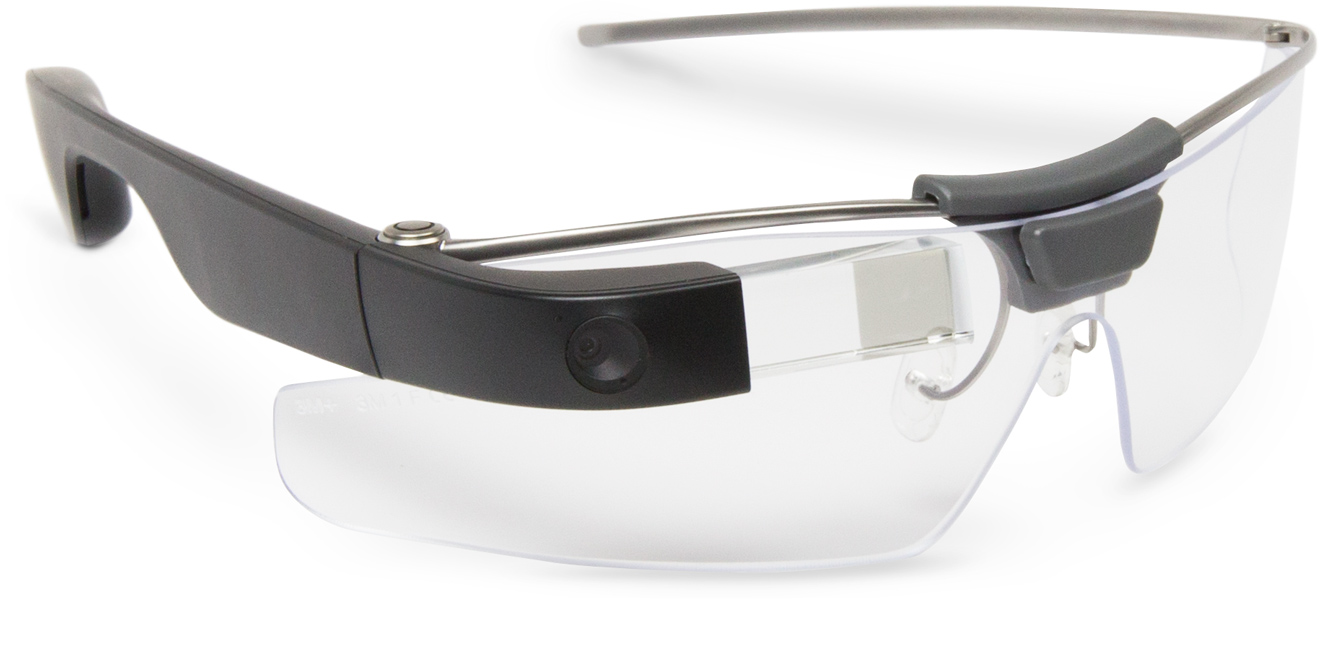
\includegraphics[width=\linewidth]{img/glass_wearable.jpeg}\\
            }
        \end{column}
        \begin{column}{.5\linewidth}
            \centering
            \begin{tikzpicture}[align=center,
    node distance=0.7cm and 0.7cm,
    every initial by arrow/.style={draw=none, minimum size=0em},
    %node styles:
    block_center/.style ={rectangle, draw=black, thick, fill=white,
            text width=8em, text centered, minimum height=4em},
    block_left/.style ={rectangle, draw=black, thick, fill=white,
            text width=16em, text ragged, minimum height=4em, inner sep=6pt},
    block_noborder/.style ={rectangle, draw=none, thick, fill=none,
            text width=18em, text centered, minimum height=1em},
    block_assign/.style ={rectangle, draw=black, thick, fill=white,
            text width=18em, text ragged, minimum height=3em, inner sep=6pt},
    block_lost/.style ={rectangle, draw=black, thick, fill=white,
            text width=16em, text ragged, minimum height=3em, inner sep=6pt},
    block_rounded/.style ={rectangle, draw=black, thick, fill=white,
            text width=8em, text centered, rounded corners=.55cm, minimum height=4em},
    line/.style ={draw, very thick, line cap=round, -{Latex[length=2.5mm]}, shorten >=0pt}
    ]

    \matrix [column sep=20mm,row sep=3mm] (mtx) {
        \node[inner sep=0pt] (user) {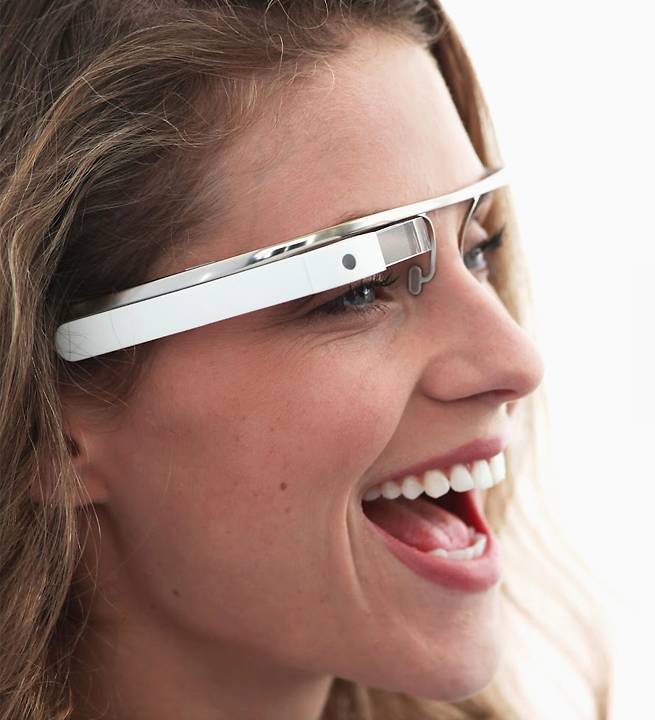
\includegraphics[height=.2\textheight]{img/google-glass.png}};
         & \node [inner sep=0pt] (server) {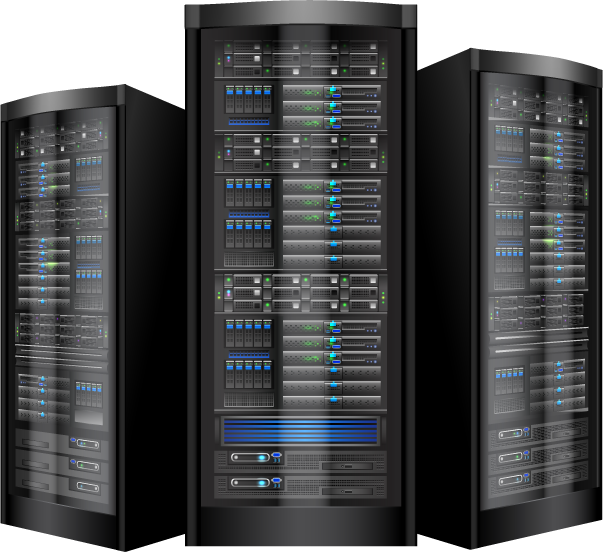
\includegraphics[height=.2\textheight]{img/server.png}}; \\
    };


    \path[draw, line]
    (user) edge [out=45, in=135] node[above] {Sensory Input} (server)
    (server) edge [out=225, in=315] node[below] {Human-parseable\\Feedback} (user);
\end{tikzpicture}%
        \end{column}%
        \begin{column}{.25\linewidth}
            \centering%
            \onslide<3->{
                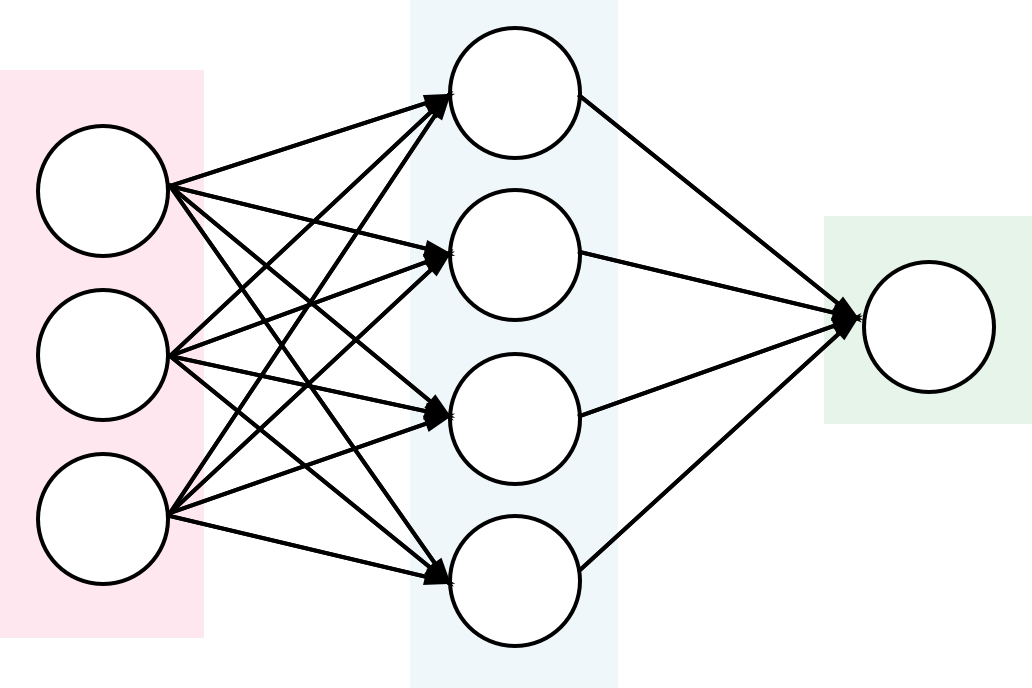
\includegraphics[width=\linewidth]{img/NN.png}\\
            }
        \end{column}%
    \end{columns}%
    \onslide<2->{\begin{columns}[onlytextwidth]
        \begin{column}{.335\linewidth}%filler
        \end{column}%
        \begin{column}{.1\linewidth}
            \centering%
            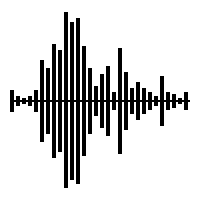
\includegraphics[width=\linewidth]{img/sound_wave.png}
        \end{column}%
        \begin{column}{.01\linewidth}
        \end{column}%
        \begin{column}{.1\linewidth}
            \centering%
            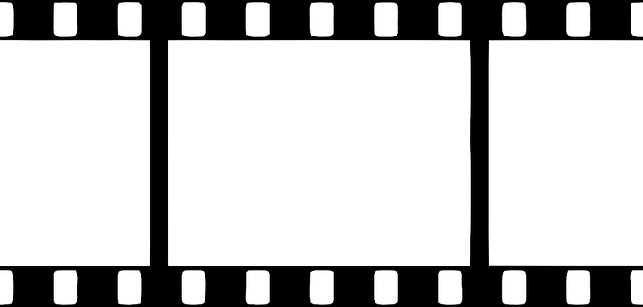
\includegraphics[width=\linewidth]{img/film.png}
        \end{column}%
        \begin{column}{.01\linewidth}
        \end{column}%
        \begin{column}{.1\linewidth}
            \centering%
            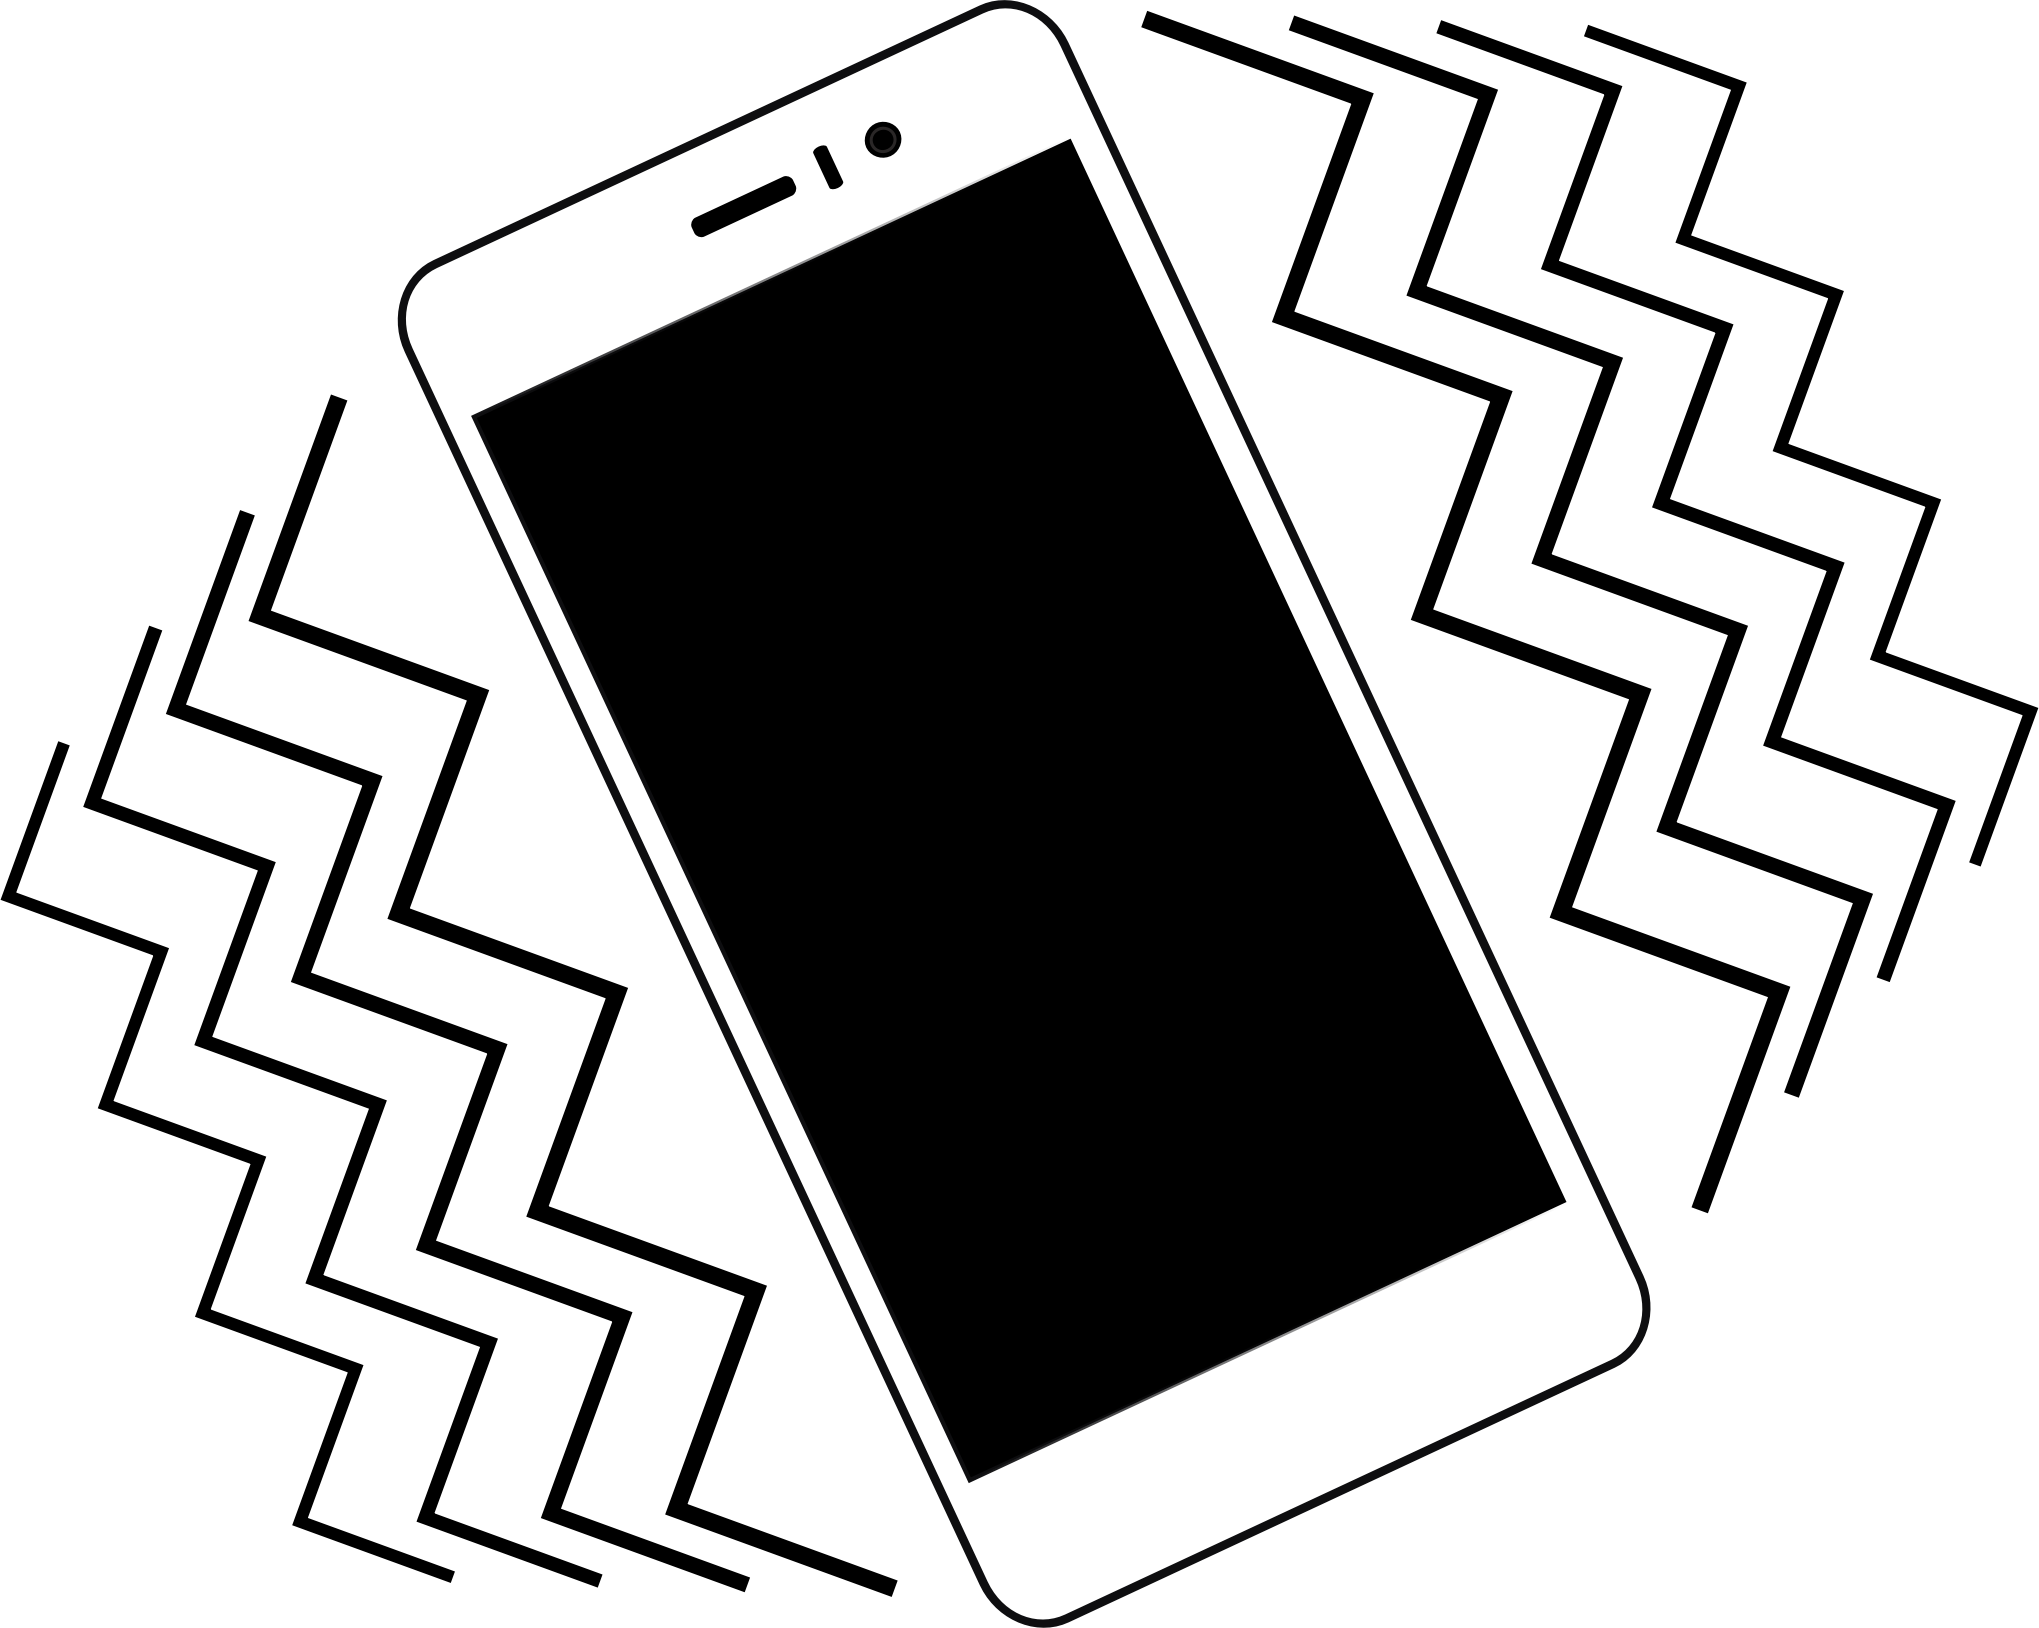
\includegraphics[width=\linewidth]{img/vibration.png}
        \end{column}%
        \begin{column}{.335\linewidth}%filler
        \end{column}}%
    \end{columns}
\end{frame}

\subsection{The Problem}
\begin{frame}{The Problem}
    \begin{Large}
        \centering%
        Benchmarking human-in-the-loop applications is HARD\\
    \end{Large}
\end{frame}
\section{Experimentally Benchmarking Human-in-the-Loop}
\subsection{Approach}

\begin{frame}{Approach: Motivation}
    \begin{center}
        \only<1>{\begin{tikzpicture}[align=center,
    node distance=0.7cm and 0.7cm,
    every initial by arrow/.style={draw=none, minimum size=0em},
    %node styles:
    block_center/.style ={rectangle, draw=black, thick, fill=white,
            text width=8em, text centered, minimum height=4em},
    block_left/.style ={rectangle, draw=black, thick, fill=white,
            text width=16em, text ragged, minimum height=4em, inner sep=6pt},
    block_noborder/.style ={rectangle, draw=none, thick, fill=none,
            text width=18em, text centered, minimum height=1em},
    block_assign/.style ={rectangle, draw=black, thick, fill=white,
            text width=18em, text ragged, minimum height=3em, inner sep=6pt},
    block_lost/.style ={rectangle, draw=black, thick, fill=white,
            text width=16em, text ragged, minimum height=3em, inner sep=6pt},
    block_rounded/.style ={rectangle, draw=black, thick, fill=white,
            text width=8em, text centered, rounded corners=.55cm, minimum height=4em},
    line/.style ={draw, very thick, line cap=round, -{Latex[length=2.5mm]}, shorten >=0pt}
    ]

    \matrix [column sep=20mm,row sep=3mm] (mtx) {
        \node[inner sep=0pt] (user) {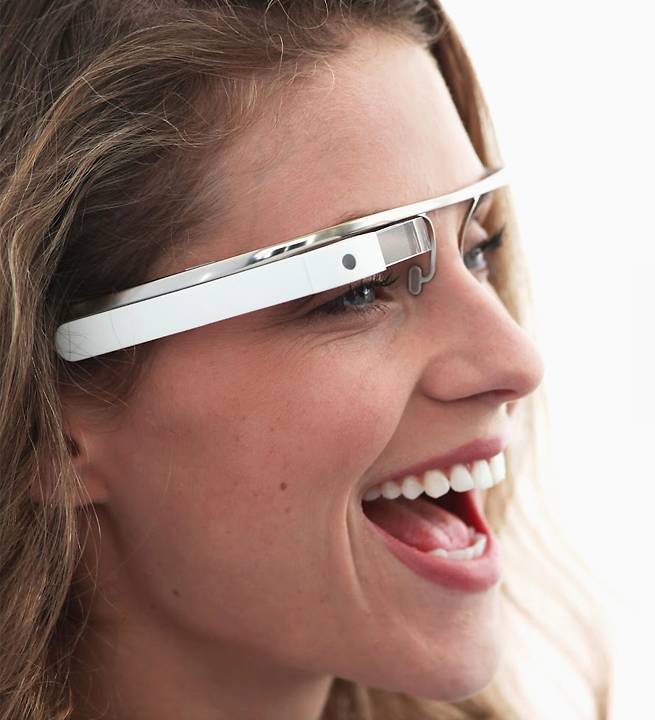
\includegraphics[height=.2\textheight]{img/google-glass.png}};
         & \node [inner sep=0pt] (server) {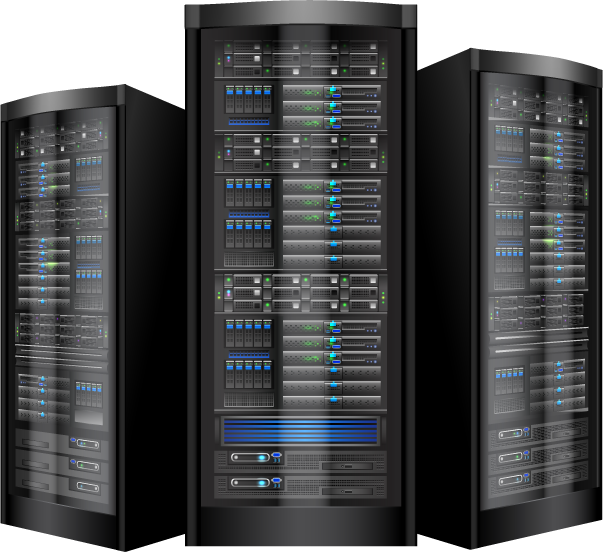
\includegraphics[height=.2\textheight]{img/server.png}}; \\
    };


    \path[draw, line]
    (user) edge [out=45, in=135] node[above] {Sensory Input} (server)
    (server) edge [out=225, in=315] node[below] {Human-parseable\\Feedback} (user);
\end{tikzpicture}}%
        \only<2>{%
            \begin{tikzpicture}[align=center,
    node distance=0.7cm and 0.7cm,
    every initial by arrow/.style={draw=none, minimum size=0em},
    %node styles:
    block_center/.style ={rectangle, draw=black, thick, fill=white,
            text width=8em, text centered, minimum height=4em},
    block_left/.style ={rectangle, draw=black, thick, fill=white,
            text width=16em, text ragged, minimum height=4em, inner sep=6pt},
    block_noborder/.style ={rectangle, draw=none, thick, fill=none,
            text width=18em, text centered, minimum height=1em},
    block_assign/.style ={rectangle, draw=black, thick, fill=white,
            text width=18em, text ragged, minimum height=3em, inner sep=6pt},
    block_lost/.style ={rectangle, draw=black, thick, fill=white,
            text width=16em, text ragged, minimum height=3em, inner sep=6pt},
    block_rounded/.style ={rectangle, draw=black, thick, fill=white,
            text width=8em, text centered, rounded corners=.55cm, minimum height=4em},
    line/.style ={draw, very thick, line cap=round, -{Latex[length=2.5mm]}, shorten >=0pt}
    ]

    \matrix [column sep=20mm,row sep=3mm] (mtx) {
        \node[inner sep=0pt] (user) {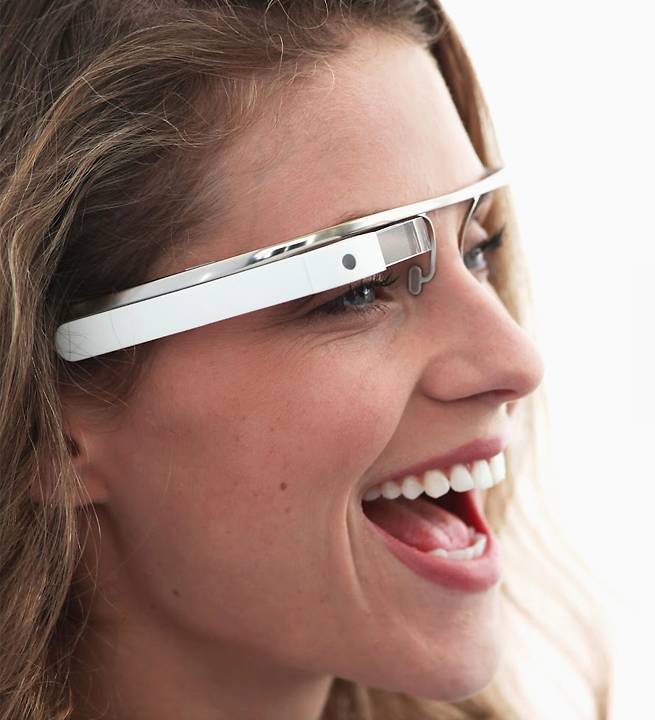
\includegraphics[height=.2\textheight]{img/google-glass.png}};
         & \node [inner sep=0pt] (server) {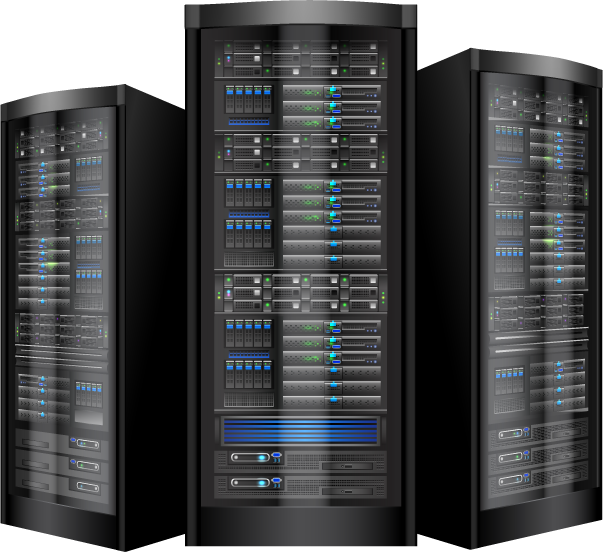
\includegraphics[height=.2\textheight]{img/server.png}}; \\
    };


    \path[draw, line]
    (user) edge [out=45, in=135] node[above] {Sensory Input} (server)
    (server) edge [out=225, in=315] node[below] {Human-parseable\\Feedback} (user);

    \draw[red, line width=2mm, line cap=round]
    (user.south west) -- (user.north east)
    (user.south east) -- (user.north west);
\end{tikzpicture}%
        }%
        \only<3>{%
            \begin{tikzpicture}[align=center,
    node distance=0.7cm and 0.7cm,
    every initial by arrow/.style={draw=none, minimum size=0em},
    %node styles:
    block_center/.style ={rectangle, draw=black, thick, fill=white,
            text width=8em, text centered, minimum height=4em},
    block_left/.style ={rectangle, draw=black, thick, fill=white,
            text width=16em, text ragged, minimum height=4em, inner sep=6pt},
    block_noborder/.style ={rectangle, draw=none, thick, fill=none,
            text width=18em, text centered, minimum height=1em},
    block_assign/.style ={rectangle, draw=black, thick, fill=white,
            text width=18em, text ragged, minimum height=3em, inner sep=6pt},
    block_lost/.style ={rectangle, draw=black, thick, fill=white,
            text width=16em, text ragged, minimum height=3em, inner sep=6pt},
    block_rounded/.style ={rectangle, draw=black, thick, fill=white,
            text width=8em, text centered, rounded corners=.55cm, minimum height=4em},
    line/.style ={draw, very thick, line cap=round, -{Latex[length=2.5mm]}, shorten >=0pt}
    ]

    \matrix [column sep=20mm,row sep=3mm] (mtx) {
        \node[inner sep=0pt] (user) {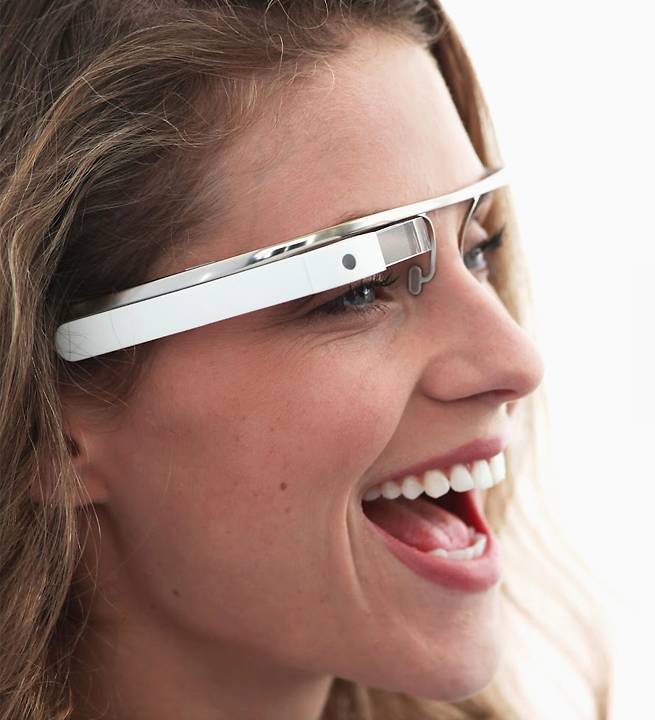
\includegraphics[height=.2\textheight]{img/google-glass.png}};
         & \node [inner sep=0pt] (server) {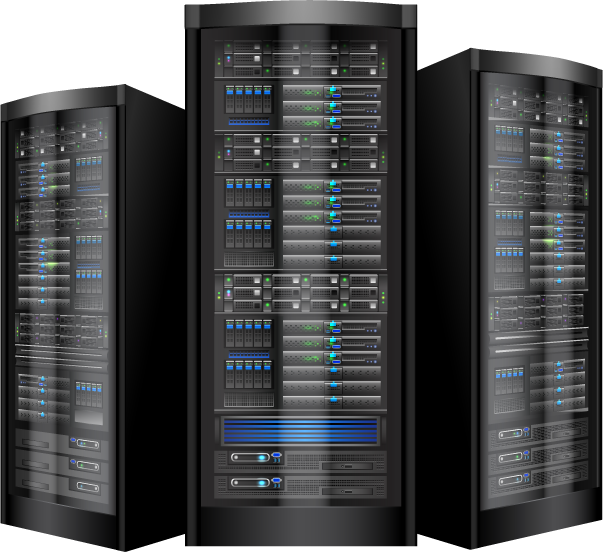
\includegraphics[height=.2\textheight]{img/server.png}}; \\
    };


    \path[draw, line]
    (user) edge [out=45, in=135] node[above] {Sensory Input} (server)
    (server) edge [out=225, in=315] node[below] {Human-parseable\\Feedback} (user);

    \draw[red, line width=2mm, line cap=round]
    (user.south west) -- (user.north east)
    (user.south east) -- (user.north west);
\end{tikzpicture}%
        }%
        %\only<3>{%
        %\input{}%
        %}%
        \onslide<2->{%
            \\\vspace{.1\textheight}%
            What if we could do away with the human user?%
        }
    \end{center}
\end{frame}

\begin{frame}{EdgeDroid: Idea}
    \begin{columns}[onlytextwidth]
        \begin{column}{.5\linewidth}
            \begin{itemize}
                \itemsep2em
                \item Generate realistic, real-time inputs.
                \onslide<2->{\begin{itemize}
                    \item Trace of human-generated inputs.
                \end{itemize}}
                \item Correctly react to feedback.
                \onslide<2->{\begin{itemize}
                    \item Model of human interaction.
                \end{itemize}}
            \end{itemize}
        \end{column}%
        \begin{column}{.5\linewidth}
            \centering%
            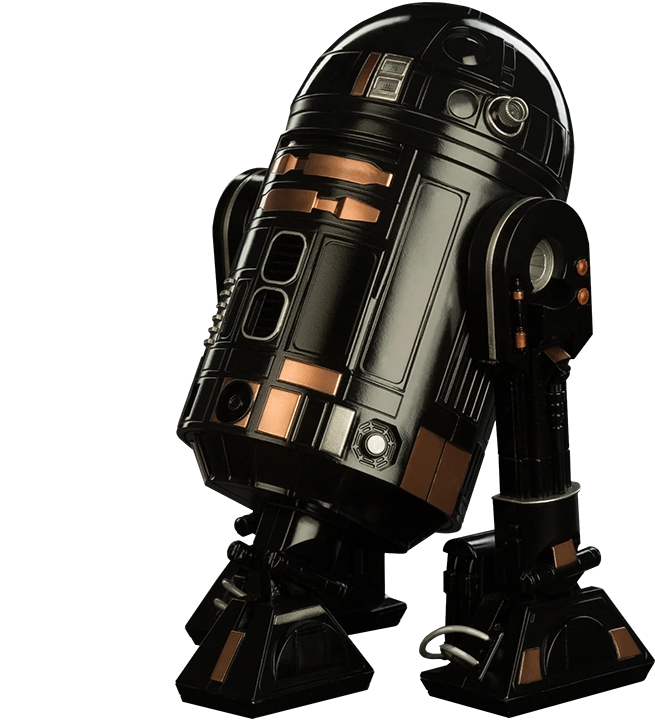
\includegraphics[width=.7\linewidth]{img/astromech.png}
        \end{column}
    \end{columns}
\end{frame}

\begin{frame}{EdgeDroid: Tracing}
    \begin{center}
        \begin{tikzpicture}[align=center, node distance=0.7cm and 0.7cm,
    line/.style ={draw, very thick, line cap=round, -{Latex[length=2.5mm]}, shorten >=0pt}]
    \matrix [column sep=4mm,row sep=10mm] (mtx) {
        & \node[draw, circle, minimum height=17mm, fill=white!60!red,
            minimum width=17mm, anchor=center] (record) {Recorder};
        & \node[inner sep=0pt] (trace) {
\includegraphics[height=.12\textheight]{img/floppy.png}\\Trace}; \\


        \node[inner sep=0pt] (user) {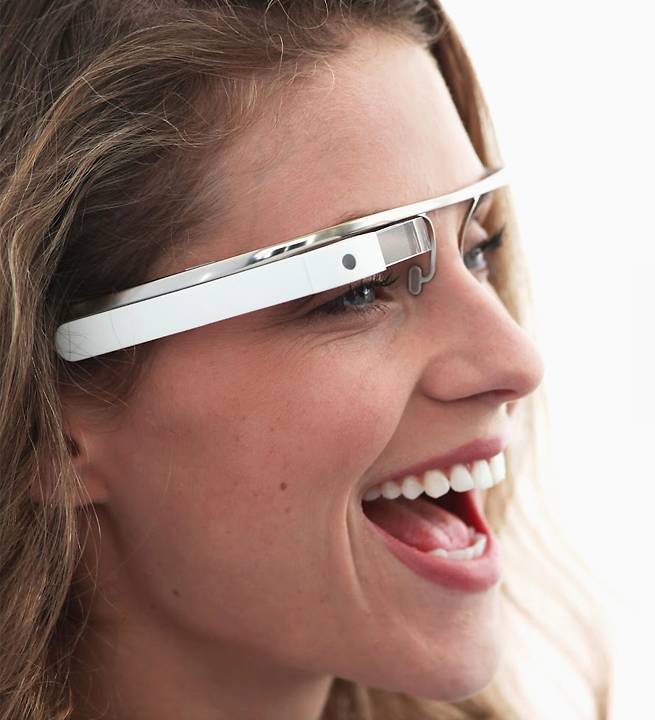
\includegraphics[height=.2\textheight]{img/google-glass.png}};
         & \node[draw=black, fill=white!80!orange, thick, single arrow, minimum height=33mm,
            minimum width=16mm, single arrow head extend=2mm, anchor=center] (inputs) {Sensory inputs};
         & \node [inner sep=0pt] (server) {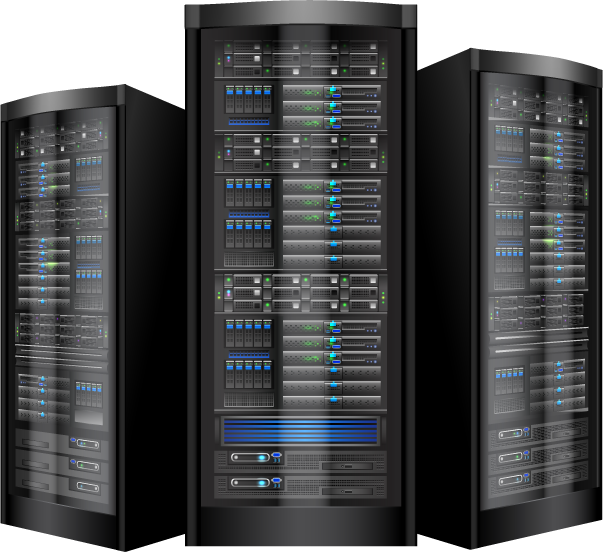
\includegraphics[height=.2\textheight]{img/server.png}}; \\
    };

    \path[draw, line]
    (record) edge node {} (trace)
    (inputs) edge node {} (record);

    %\draw[thick, line cap=round, -{Latex[length=2.5mm]}, shorten >=0pt]
    %(record.east) -- (trace.west);


    %(inputs.north) -- (record.south);

    %\draw[white!30!violet, line width=.5mm, line cap=round]
    %(inputs.160) -- (record.225)
    %(inputs.20) -- (record.315);
\end{tikzpicture}\\
    \end{center}
\end{frame}

\begin{frame}{EdgeDroid: User Model}
    \begin{center}
        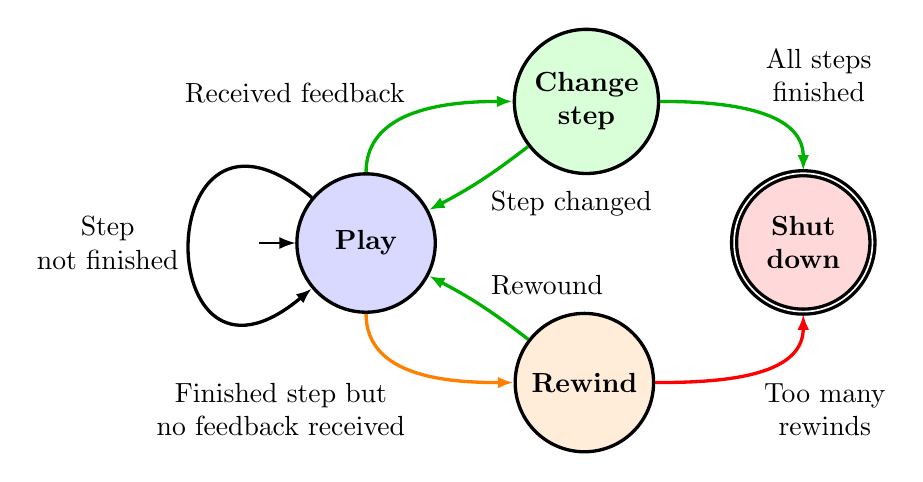
\begin{tikzpicture}[align=center,
    node distance=.5cm and 1.5cm,
    every initial by arrow/.style={-{Latex[length=2mm]}}]
    % Place nodes              
    \node [initial, very thick, state, minimum size=5em, initial text=, fill=white!85!blue] (play) {\textbf{Play}};
    \node [state, very thick, above right=of play, minimum size=5em, fill=white!85!green] (change) {\textbf{Change}\\\textbf{step}};
    \node [state, very thick, below right=of play, minimum size=5em, fill=white!85!orange] (rewind) {\textbf{Rewind}};
    \node [state, very thick, accepting, above right=of rewind, minimum size=5em, fill=white!85!red] (shutdown) {\textbf{Shut}\\\textbf{down}};

    % Draw edges
    \path[draw, -{Latex[length=2mm]}, very thick]
    (play) edge [out=270, in=180, color=red!50!yellow] node[below left, color=black] {Finished step but\\no feedback received} (rewind)
    edge [out=90, in=180, color=black!30!green] node[above left, color=black] {Received feedback} (change)
    edge [out=140, in=220,looseness=6] node[left] {Step\\not finished} (play)

    (change) edge [bend left=5, color=black!30!green] node[below right, color=black] {Step changed} (play)
    edge [out=0, in=90, color=black!30!green] node[above right, color=black] {All steps\\finished} (shutdown)

    (rewind) edge [bend right=5, color=black!30!green] node[above right, color=black] {Rewound} (play)
    edge [out=0, in=270, color=red] node[below right, color=black] {Too many\\rewinds} (shutdown);

\end{tikzpicture}\\
    \end{center}
\end{frame}

\begin{frame}{Implementation}
    \begin{center}
        \begin{tikzpicture}[align=center, font={\footnotesize},
    arrow/.style={draw, thick, -{Latex[length=2mm]}},
    arrowr/.style={draw, thick, {Latex[length=2mm]}-},
    parallelogram/.style={trapezium,trapezium left angle=70,trapezium right angle=-70}]

    % layers
    \pgfdeclarelayer{background0}
    \pgfdeclarelayer{background1}
    \pgfdeclarelayer{foreground}
    \pgfsetlayers{background0,background1,foreground}
    
    \begin{pgfonlayer}{foreground}
        \matrix[column sep=40mm, row sep=2mm, inner sep=2mm,
        every node/.style={text width=4em, text centered, minimum width=5em}] (mtx) {
            \node[dashed, draw, rectangle, anchor=center, inner sep=2mm, ] (usermodel) {``User''\\Model}; 
            & \node[draw, dashed, rectangle, anchor=center, inner sep=2mm] (app_backend) {App Backend};\\

            \node[inner sep=0mm] {}; %spacer
            & \node[anchor=center, inner sep=0mm] (docker) {Container};\\

            % spacers
            \node[inner sep=0mm, minimum height=1.5em] {};
            & \node[inner sep=0mm, minimum height=1.5em] {}; \\

            \node[anchor=center, inner sep=2mm, minimum height=5em] (emulator) {Client Emulator\\Java 1.8};
            & \node[anchor=center, inner sep=2mm, minimum height=5em] (control) {Control Backend\\Python 3.6};\\

            % spacers
            \node[inner sep=0mm, minimum height=.5em] {};
            & \node[inner sep=0mm, minimum height=.5em] {}; \\

            \node[inner sep=0mm, minimum height=2em] (label1_padding) {}; 
            & \node[inner sep=0mm, minimum height=2em] (label2_padding) {}; \\
        };

        \node[parallelogram, draw, inner sep=2mm, right=10mm of control.25, 
        minimum width=20mm, minimum height=2em, fill=white!80!violet] (config) {Config};
        \node[parallelogram, draw, inner sep=2mm, right=10mm of control.335, 
        minimum width=20mm, minimum height=2em, fill=white!80!violet] (trace) {Trace};
    \end{pgfonlayer}

    \begin{pgfonlayer}{background1}
        \node[fit=(usermodel) (emulator), draw, fill=white!80!yellow] (fit1) {};
        %\node[fit=(app_backend) (control)] (fit2) {};
        \node[fit=(docker) (app_backend), draw, fill=white!80!blue] (fit3) {};
        \node[fit=(control), draw, fill=white!80!red] (fit_control) {}; % just to make the size match
    \end{pgfonlayer}

    % main background fits
    \begin{pgfonlayer}{background0}
        \node[fit=(label1_padding) (fit1), draw, fill=white!80!green] (android) {};
        \node[fit=(label2_padding) (fit_control) (fit3) (config.top right corner) (trace.top right corner), draw, fill=white!80!black] (cloudlet) {};
    \end{pgfonlayer}

    \begin{pgfonlayer}{foreground}
        % primary labels
        \node[inner sep=2mm, above] at (android.south) {Android\\6.0+};
        \node[inner sep=2mm, above] at (cloudlet.south) {Cloudlet\\Linux v4.13.0+};


        % arrows
        % config and trace
        \draw[arrow] (config.west) -- (config.west -| fit_control.east);
        \draw[arrow] (trace.west) -- (trace.west -| fit_control.east);

        % between app and control backend
        \draw[arrowr] (fit_control.95) -- (fit_control.95 |- fit3.south);
        \draw[arrow] (fit_control.85) -- node[right] {\footnotesize Execution Control} (fit_control.85 |- fit3.south);

        % between app and user model
        \coordinate (a1) at (app_backend.165 -| fit3.west);
        \coordinate (a2) at (app_backend.195 -| fit3.west);
        \coordinate (b1) at (a1 -| fit1.east);
        \coordinate (b2) at (a2 -| fit1.east);

        \draw[arrow] (a1) -- coordinate[midway] (ab1) (b1);
        \draw[arrowr] (a2) -- coordinate[midway] (ab2) (b2);
        \path (ab1) -- node[midway, anchor=center, inner sep=0mm] {Feedback Loop} (ab2); % center label between arrows

        % between control and client
        \draw[arrow, dashed] (fit_control.155) -- node[above] {Config, Trace} node[below] {\tiny Before experiment} (fit_control.155 -| fit1.east);
        \draw[arrowr, dashed] (fit_control.205) -- node[above] {Results} node[below] {\tiny After experiment} (fit_control.205 -| fit1.east);
    \end{pgfonlayer}

\end{tikzpicture}
    \end{center}
\end{frame}

\begin{frame}{Evaluation}

\end{frame}


\subsection{Implementation}
\subsection{Evaluation}
\section{Conclusions}

\end{document}